% Graphic for TeX using PGF
% Title: /home/satenske/cours/AP/obj3/TD1/3.dia
% Creator: Dia v0.97.1
% CreationDate: Thu Oct 20 09:25:31 2011
% For: satenske
% \usepackage{tikz}
% The following commands are not supported in PSTricks at present
% We define them conditionally, so when they are implemented,
% this pgf file will use them.
\ifx\du\undefined
  \newlength{\du}
\fi
\setlength{\du}{15\unitlength}
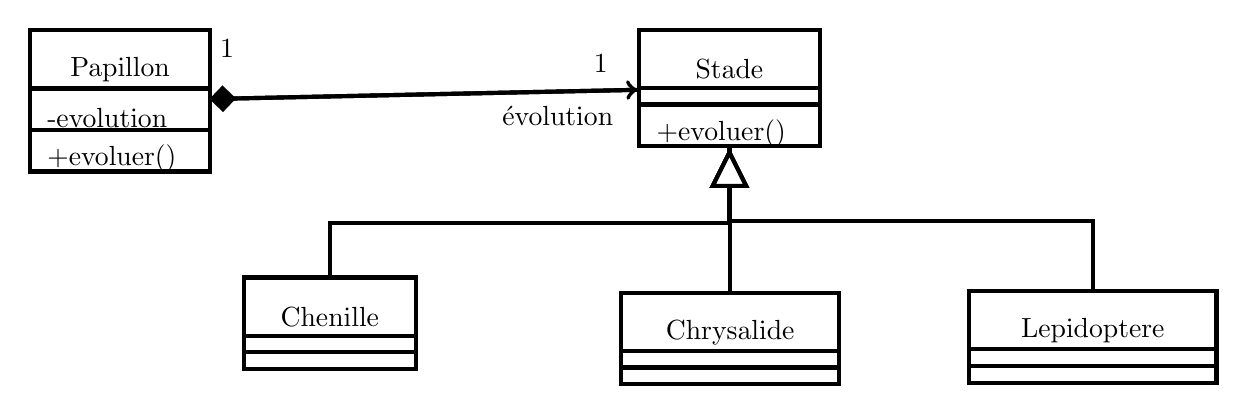
\begin{tikzpicture}
\pgftransformxscale{1.000000}
\pgftransformyscale{-1.000000}
\definecolor{dialinecolor}{rgb}{0.000000, 0.000000, 0.000000}
\pgfsetstrokecolor{dialinecolor}
\definecolor{dialinecolor}{rgb}{1.000000, 1.000000, 1.000000}
\pgfsetfillcolor{dialinecolor}
\pgfsetlinewidth{0.100000\du}
\pgfsetdash{}{0pt}
\definecolor{dialinecolor}{rgb}{1.000000, 1.000000, 1.000000}
\pgfsetfillcolor{dialinecolor}
\fill (23.350000\du,2.600000\du)--(23.350000\du,4.000000\du)--(27.700000\du,4.000000\du)--(27.700000\du,2.600000\du)--cycle;
\definecolor{dialinecolor}{rgb}{0.000000, 0.000000, 0.000000}
\pgfsetstrokecolor{dialinecolor}
\draw (23.350000\du,2.600000\du)--(23.350000\du,4.000000\du)--(27.700000\du,4.000000\du)--(27.700000\du,2.600000\du)--cycle;
% setfont left to latex
\definecolor{dialinecolor}{rgb}{0.000000, 0.000000, 0.000000}
\pgfsetstrokecolor{dialinecolor}
\node at (25.525000\du,3.550000\du){Papillon};
\definecolor{dialinecolor}{rgb}{1.000000, 1.000000, 1.000000}
\pgfsetfillcolor{dialinecolor}
\fill (23.350000\du,4.000000\du)--(23.350000\du,5.000000\du)--(27.700000\du,5.000000\du)--(27.700000\du,4.000000\du)--cycle;
\definecolor{dialinecolor}{rgb}{0.000000, 0.000000, 0.000000}
\pgfsetstrokecolor{dialinecolor}
\draw (23.350000\du,4.000000\du)--(23.350000\du,5.000000\du)--(27.700000\du,5.000000\du)--(27.700000\du,4.000000\du)--cycle;
% setfont left to latex
\definecolor{dialinecolor}{rgb}{0.000000, 0.000000, 0.000000}
\pgfsetstrokecolor{dialinecolor}
\node[anchor=west] at (23.500000\du,4.700000\du){-evolution};
\definecolor{dialinecolor}{rgb}{1.000000, 1.000000, 1.000000}
\pgfsetfillcolor{dialinecolor}
\fill (23.350000\du,5.000000\du)--(23.350000\du,6.000000\du)--(27.700000\du,6.000000\du)--(27.700000\du,5.000000\du)--cycle;
\definecolor{dialinecolor}{rgb}{0.000000, 0.000000, 0.000000}
\pgfsetstrokecolor{dialinecolor}
\draw (23.350000\du,5.000000\du)--(23.350000\du,6.000000\du)--(27.700000\du,6.000000\du)--(27.700000\du,5.000000\du)--cycle;
% setfont left to latex
\definecolor{dialinecolor}{rgb}{0.000000, 0.000000, 0.000000}
\pgfsetstrokecolor{dialinecolor}
\node[anchor=west] at (23.500000\du,5.700000\du){+evoluer()};
\pgfsetlinewidth{0.100000\du}
\pgfsetdash{}{0pt}
\definecolor{dialinecolor}{rgb}{1.000000, 1.000000, 1.000000}
\pgfsetfillcolor{dialinecolor}
\fill (45.980000\du,8.885000\du)--(45.980000\du,10.285000\du)--(51.937500\du,10.285000\du)--(51.937500\du,8.885000\du)--cycle;
\definecolor{dialinecolor}{rgb}{0.000000, 0.000000, 0.000000}
\pgfsetstrokecolor{dialinecolor}
\draw (45.980000\du,8.885000\du)--(45.980000\du,10.285000\du)--(51.937500\du,10.285000\du)--(51.937500\du,8.885000\du)--cycle;
% setfont left to latex
\definecolor{dialinecolor}{rgb}{0.000000, 0.000000, 0.000000}
\pgfsetstrokecolor{dialinecolor}
\node at (48.958750\du,9.835000\du){Lepidoptere};
\definecolor{dialinecolor}{rgb}{1.000000, 1.000000, 1.000000}
\pgfsetfillcolor{dialinecolor}
\fill (45.980000\du,10.285000\du)--(45.980000\du,10.685000\du)--(51.937500\du,10.685000\du)--(51.937500\du,10.285000\du)--cycle;
\definecolor{dialinecolor}{rgb}{0.000000, 0.000000, 0.000000}
\pgfsetstrokecolor{dialinecolor}
\draw (45.980000\du,10.285000\du)--(45.980000\du,10.685000\du)--(51.937500\du,10.685000\du)--(51.937500\du,10.285000\du)--cycle;
\definecolor{dialinecolor}{rgb}{1.000000, 1.000000, 1.000000}
\pgfsetfillcolor{dialinecolor}
\fill (45.980000\du,10.685000\du)--(45.980000\du,11.085000\du)--(51.937500\du,11.085000\du)--(51.937500\du,10.685000\du)--cycle;
\definecolor{dialinecolor}{rgb}{0.000000, 0.000000, 0.000000}
\pgfsetstrokecolor{dialinecolor}
\draw (45.980000\du,10.685000\du)--(45.980000\du,11.085000\du)--(51.937500\du,11.085000\du)--(51.937500\du,10.685000\du)--cycle;
\pgfsetlinewidth{0.100000\du}
\pgfsetdash{}{0pt}
\definecolor{dialinecolor}{rgb}{1.000000, 1.000000, 1.000000}
\pgfsetfillcolor{dialinecolor}
\fill (37.595000\du,8.920000\du)--(37.595000\du,10.320000\du)--(42.850000\du,10.320000\du)--(42.850000\du,8.920000\du)--cycle;
\definecolor{dialinecolor}{rgb}{0.000000, 0.000000, 0.000000}
\pgfsetstrokecolor{dialinecolor}
\draw (37.595000\du,8.920000\du)--(37.595000\du,10.320000\du)--(42.850000\du,10.320000\du)--(42.850000\du,8.920000\du)--cycle;
% setfont left to latex
\definecolor{dialinecolor}{rgb}{0.000000, 0.000000, 0.000000}
\pgfsetstrokecolor{dialinecolor}
\node at (40.222500\du,9.870000\du){Chrysalide};
\definecolor{dialinecolor}{rgb}{1.000000, 1.000000, 1.000000}
\pgfsetfillcolor{dialinecolor}
\fill (37.595000\du,10.320000\du)--(37.595000\du,10.720000\du)--(42.850000\du,10.720000\du)--(42.850000\du,10.320000\du)--cycle;
\definecolor{dialinecolor}{rgb}{0.000000, 0.000000, 0.000000}
\pgfsetstrokecolor{dialinecolor}
\draw (37.595000\du,10.320000\du)--(37.595000\du,10.720000\du)--(42.850000\du,10.720000\du)--(42.850000\du,10.320000\du)--cycle;
\definecolor{dialinecolor}{rgb}{1.000000, 1.000000, 1.000000}
\pgfsetfillcolor{dialinecolor}
\fill (37.595000\du,10.720000\du)--(37.595000\du,11.120000\du)--(42.850000\du,11.120000\du)--(42.850000\du,10.720000\du)--cycle;
\definecolor{dialinecolor}{rgb}{0.000000, 0.000000, 0.000000}
\pgfsetstrokecolor{dialinecolor}
\draw (37.595000\du,10.720000\du)--(37.595000\du,11.120000\du)--(42.850000\du,11.120000\du)--(42.850000\du,10.720000\du)--cycle;
\pgfsetlinewidth{0.100000\du}
\pgfsetdash{}{0pt}
\definecolor{dialinecolor}{rgb}{1.000000, 1.000000, 1.000000}
\pgfsetfillcolor{dialinecolor}
\fill (28.510000\du,8.555000\du)--(28.510000\du,9.955000\du)--(32.647500\du,9.955000\du)--(32.647500\du,8.555000\du)--cycle;
\definecolor{dialinecolor}{rgb}{0.000000, 0.000000, 0.000000}
\pgfsetstrokecolor{dialinecolor}
\draw (28.510000\du,8.555000\du)--(28.510000\du,9.955000\du)--(32.647500\du,9.955000\du)--(32.647500\du,8.555000\du)--cycle;
% setfont left to latex
\definecolor{dialinecolor}{rgb}{0.000000, 0.000000, 0.000000}
\pgfsetstrokecolor{dialinecolor}
\node at (30.578750\du,9.505000\du){Chenille};
\definecolor{dialinecolor}{rgb}{1.000000, 1.000000, 1.000000}
\pgfsetfillcolor{dialinecolor}
\fill (28.510000\du,9.955000\du)--(28.510000\du,10.355000\du)--(32.647500\du,10.355000\du)--(32.647500\du,9.955000\du)--cycle;
\definecolor{dialinecolor}{rgb}{0.000000, 0.000000, 0.000000}
\pgfsetstrokecolor{dialinecolor}
\draw (28.510000\du,9.955000\du)--(28.510000\du,10.355000\du)--(32.647500\du,10.355000\du)--(32.647500\du,9.955000\du)--cycle;
\definecolor{dialinecolor}{rgb}{1.000000, 1.000000, 1.000000}
\pgfsetfillcolor{dialinecolor}
\fill (28.510000\du,10.355000\du)--(28.510000\du,10.755000\du)--(32.647500\du,10.755000\du)--(32.647500\du,10.355000\du)--cycle;
\definecolor{dialinecolor}{rgb}{0.000000, 0.000000, 0.000000}
\pgfsetstrokecolor{dialinecolor}
\draw (28.510000\du,10.355000\du)--(28.510000\du,10.755000\du)--(32.647500\du,10.755000\du)--(32.647500\du,10.355000\du)--cycle;
\pgfsetlinewidth{0.100000\du}
\pgfsetdash{}{0pt}
\definecolor{dialinecolor}{rgb}{1.000000, 1.000000, 1.000000}
\pgfsetfillcolor{dialinecolor}
\fill (38.030000\du,2.585000\du)--(38.030000\du,3.985000\du)--(42.380000\du,3.985000\du)--(42.380000\du,2.585000\du)--cycle;
\definecolor{dialinecolor}{rgb}{0.000000, 0.000000, 0.000000}
\pgfsetstrokecolor{dialinecolor}
\draw (38.030000\du,2.585000\du)--(38.030000\du,3.985000\du)--(42.380000\du,3.985000\du)--(42.380000\du,2.585000\du)--cycle;
% setfont left to latex
\definecolor{dialinecolor}{rgb}{0.000000, 0.000000, 0.000000}
\pgfsetstrokecolor{dialinecolor}
\node at (40.205000\du,3.535000\du){Stade};
\definecolor{dialinecolor}{rgb}{1.000000, 1.000000, 1.000000}
\pgfsetfillcolor{dialinecolor}
\fill (38.030000\du,3.985000\du)--(38.030000\du,4.385000\du)--(42.380000\du,4.385000\du)--(42.380000\du,3.985000\du)--cycle;
\definecolor{dialinecolor}{rgb}{0.000000, 0.000000, 0.000000}
\pgfsetstrokecolor{dialinecolor}
\draw (38.030000\du,3.985000\du)--(38.030000\du,4.385000\du)--(42.380000\du,4.385000\du)--(42.380000\du,3.985000\du)--cycle;
\definecolor{dialinecolor}{rgb}{1.000000, 1.000000, 1.000000}
\pgfsetfillcolor{dialinecolor}
\fill (38.030000\du,4.385000\du)--(38.030000\du,5.385000\du)--(42.380000\du,5.385000\du)--(42.380000\du,4.385000\du)--cycle;
\definecolor{dialinecolor}{rgb}{0.000000, 0.000000, 0.000000}
\pgfsetstrokecolor{dialinecolor}
\draw (38.030000\du,4.385000\du)--(38.030000\du,5.385000\du)--(42.380000\du,5.385000\du)--(42.380000\du,4.385000\du)--cycle;
% setfont left to latex
\definecolor{dialinecolor}{rgb}{0.000000, 0.000000, 0.000000}
\pgfsetstrokecolor{dialinecolor}
\node[anchor=west] at (38.180000\du,5.085000\du){+evoluer()};
\pgfsetlinewidth{0.100000\du}
\pgfsetdash{}{0pt}
\pgfsetdash{}{0pt}
\pgfsetbuttcap
{
\definecolor{dialinecolor}{rgb}{0.000000, 0.000000, 0.000000}
\pgfsetfillcolor{dialinecolor}
% was here!!!
\pgfsetarrowsend{to}
\definecolor{dialinecolor}{rgb}{0.000000, 0.000000, 0.000000}
\pgfsetstrokecolor{dialinecolor}
\draw (27.748862\du,4.252281\du)--(37.981138\du,4.032719\du);
}
\definecolor{dialinecolor}{rgb}{0.000000, 0.000000, 0.000000}
\pgfsetstrokecolor{dialinecolor}
\draw (28.107358\du,4.244588\du)--(37.981138\du,4.032719\du);
\pgfsetdash{}{0pt}
\pgfsetmiterjoin
\pgfsetbuttcap
\definecolor{dialinecolor}{rgb}{0.000000, 0.000000, 0.000000}
\pgfsetfillcolor{dialinecolor}
\fill (27.748862\du,4.252281\du)--(27.993442\du,3.996975\du)--(28.248747\du,4.241554\du)--(28.004168\du,4.496860\du)--cycle;
\pgfsetlinewidth{0.100000\du}
\pgfsetdash{}{0pt}
\pgfsetmiterjoin
\pgfsetbuttcap
\definecolor{dialinecolor}{rgb}{0.000000, 0.000000, 0.000000}
\pgfsetstrokecolor{dialinecolor}
\draw (27.748862\du,4.252281\du)--(27.993442\du,3.996975\du)--(28.248747\du,4.241554\du)--(28.004168\du,4.496860\du)--cycle;
% setfont left to latex
\definecolor{dialinecolor}{rgb}{0.000000, 0.000000, 0.000000}
\pgfsetstrokecolor{dialinecolor}
\node[anchor=west] at (27.665000\du,3.050000\du){ 1                           };
% setfont left to latex
\definecolor{dialinecolor}{rgb}{0.000000, 0.000000, 0.000000}
\pgfsetstrokecolor{dialinecolor}
\node[anchor=west] at (28.165000\du,2.800000\du){};
\pgfsetlinewidth{0.100000\du}
\pgfsetdash{}{0pt}
\pgfsetmiterjoin
\pgfsetbuttcap
{
\definecolor{dialinecolor}{rgb}{0.000000, 0.000000, 0.000000}
\pgfsetfillcolor{dialinecolor}
% was here!!!
\definecolor{dialinecolor}{rgb}{0.000000, 0.000000, 0.000000}
\pgfsetstrokecolor{dialinecolor}
\draw (40.205000\du,5.432378\du)--(40.205000\du,7.200000\du)--(48.958750\du,7.200000\du)--(48.958750\du,8.835916\du);
}
\definecolor{dialinecolor}{rgb}{0.000000, 0.000000, 0.000000}
\pgfsetstrokecolor{dialinecolor}
\draw (40.205000\du,6.344181\du)--(40.205000\du,7.200000\du)--(48.958750\du,7.200000\du)--(48.958750\du,8.835916\du);
\pgfsetmiterjoin
\definecolor{dialinecolor}{rgb}{1.000000, 1.000000, 1.000000}
\pgfsetfillcolor{dialinecolor}
\fill (40.605000\du,6.344181\du)--(40.205000\du,5.544181\du)--(39.805000\du,6.344181\du)--cycle;
\pgfsetlinewidth{0.100000\du}
\pgfsetdash{}{0pt}
\pgfsetmiterjoin
\definecolor{dialinecolor}{rgb}{0.000000, 0.000000, 0.000000}
\pgfsetstrokecolor{dialinecolor}
\draw (40.605000\du,6.344181\du)--(40.205000\du,5.544181\du)--(39.805000\du,6.344181\du)--cycle;
% setfont left to latex
\pgfsetlinewidth{0.100000\du}
\pgfsetdash{}{0pt}
\pgfsetmiterjoin
\pgfsetbuttcap
{
\definecolor{dialinecolor}{rgb}{0.000000, 0.000000, 0.000000}
\pgfsetfillcolor{dialinecolor}
% was here!!!
\definecolor{dialinecolor}{rgb}{0.000000, 0.000000, 0.000000}
\pgfsetstrokecolor{dialinecolor}
\draw (40.205000\du,5.435354\du)--(40.205000\du,7.152537\du)--(40.222500\du,7.152537\du)--(40.222500\du,8.869719\du);
}
\definecolor{dialinecolor}{rgb}{0.000000, 0.000000, 0.000000}
\pgfsetstrokecolor{dialinecolor}
\draw (40.205000\du,6.347157\du)--(40.205000\du,7.152537\du)--(40.222500\du,7.152537\du)--(40.222500\du,8.869719\du);
\pgfsetmiterjoin
\definecolor{dialinecolor}{rgb}{1.000000, 1.000000, 1.000000}
\pgfsetfillcolor{dialinecolor}
\fill (40.605000\du,6.347157\du)--(40.205000\du,5.547157\du)--(39.805000\du,6.347157\du)--cycle;
\pgfsetlinewidth{0.100000\du}
\pgfsetdash{}{0pt}
\pgfsetmiterjoin
\definecolor{dialinecolor}{rgb}{0.000000, 0.000000, 0.000000}
\pgfsetstrokecolor{dialinecolor}
\draw (40.605000\du,6.347157\du)--(40.205000\du,5.547157\du)--(39.805000\du,6.347157\du)--cycle;
% setfont left to latex
\pgfsetlinewidth{0.100000\du}
\pgfsetdash{}{0pt}
\pgfsetmiterjoin
\pgfsetbuttcap
{
\definecolor{dialinecolor}{rgb}{0.000000, 0.000000, 0.000000}
\pgfsetfillcolor{dialinecolor}
% was here!!!
\definecolor{dialinecolor}{rgb}{0.000000, 0.000000, 0.000000}
\pgfsetstrokecolor{dialinecolor}
\draw (40.205000\du,5.434163\du)--(40.205000\du,7.250000\du)--(30.578750\du,7.250000\du)--(30.578750\du,8.555000\du);
}
\definecolor{dialinecolor}{rgb}{0.000000, 0.000000, 0.000000}
\pgfsetstrokecolor{dialinecolor}
\draw (40.205000\du,6.345966\du)--(40.205000\du,7.250000\du)--(30.578750\du,7.250000\du)--(30.578750\du,8.555000\du);
\pgfsetmiterjoin
\definecolor{dialinecolor}{rgb}{1.000000, 1.000000, 1.000000}
\pgfsetfillcolor{dialinecolor}
\fill (40.605000\du,6.345966\du)--(40.205000\du,5.545966\du)--(39.805000\du,6.345966\du)--cycle;
\pgfsetlinewidth{0.100000\du}
\pgfsetdash{}{0pt}
\pgfsetmiterjoin
\definecolor{dialinecolor}{rgb}{0.000000, 0.000000, 0.000000}
\pgfsetstrokecolor{dialinecolor}
\draw (40.605000\du,6.345966\du)--(40.205000\du,5.545966\du)--(39.805000\du,6.345966\du)--cycle;
% setfont left to latex
% setfont left to latex
\definecolor{dialinecolor}{rgb}{0.000000, 0.000000, 0.000000}
\pgfsetstrokecolor{dialinecolor}
\node[anchor=west] at (36.665000\du,3.400000\du){ 1};
% setfont left to latex
\definecolor{dialinecolor}{rgb}{0.000000, 0.000000, 0.000000}
\pgfsetstrokecolor{dialinecolor}
\node[anchor=west] at (34.465000\du,4.650000\du){évolution};
\end{tikzpicture}
